\documentclass[11pt,a4paper]{article}

\usepackage[margin=1.0in]{geometry}
\usepackage{amsmath,amssymb}
\usepackage{booktabs}
\usepackage{graphicx}
\usepackage{float}
\usepackage[colorlinks=true,linkcolor=blue,urlcolor=blue,citecolor=blue]{hyperref}

\graphicspath{{../}{./}}
\setlength{\parindent}{0pt}
\setlength{\parskip}{0.55em}
\sloppy


\title{%
  \vspace{-2.5em}
  
\includegraphics[width=0.30\textwidth]{figures/pythoneers_logo.png}\\[1.4em]
  \textbf{\Large Modeling Infectious Default Risk in Basket Credit Derivatives:\\
  From First-to-Default (FTD) Swaps to $k$-th-to-Default Tranches}
}
\author{Pythoneers - The Quantitative Finance Society of Católica Lisbon \\ \\ Estêvão de Abreu Peixoto, Tomé Fernandes}
\date{October 2026}

\begin{document}

\maketitle

\begin{abstract}
\noindent
This learning note documents our end-to-end Python implementation (\texttt{hawkes\_credit.py}) of a continuous-time multivariate Hawkes point process for pricing multi-name basket credit derivatives. Starting from synthetic 5-year Credit Default Swap (CDS) spreads and a five-entity sector correlation matrix, we bootstrap baseline hazard rates $\mu_i$ alongside an off-diagonal contagion matrix $\alpha_{ij}$ with absorbing default states ($\alpha_{ii}=0$). We then simulate 10,000 exact trajectories via Ogata's modified thinning algorithm. Along the way, we highlight a critical structural insight that surfaced during development: a pure First-to-Default ($k=1$) swap is mathematically blind to post-default Hawkes contagion because all excitation jumps occur at or after $\tau_{(1)}$. Extending the Monte Carlo engine to the full capital structure of $k$-th-to-Default tranches ($k = 1, \dots, 5$) with pathwise Common Random Numbers (CRN) reveals how self-exciting sector contagion reprices mezzanine and senior basket protection by up to $+318.47\text{ bps}$.
\end{abstract}

\section{Project Scope \& Model Mechanics}

Standard textbook models for multi-name credit baskets link obligor default times through a static latent correlation parameter. While convenient for quick quoting, static copulas lack a dynamic time-series mechanism for \emph{default clustering}: in reality, when a major bank or energy producer defaults, counterparty exposures and funding freezes immediately drive up the default intensities of surviving firms in the same sector.

To model this feedback loop directly in continuous time over a $T = 5.0\text{ year}$ horizon, we track a basket of $N = 5$ corporate obligors with default stopping times $\tau_i$ and survival indicators $Y_i(t) = \mathbf{1}_{\{\tau_i > t\}}$. Prior to its own default, each entity's instantaneous hazard rate $\lambda_i(t)$ evolves as a mutually exciting Hawkes process:
\begin{equation}
  \lambda_i(t) = \mu_i + \sum_{j=1}^{N} \int_{(0, t]} \alpha_{ij} \, e^{-\beta_{ij}(t - s)} \, \mathrm{d}N_j(s)
  = \mu_i + \sum_{m : \tau_{(m)} \le t} \alpha_{i, j_{(m)}} \, e^{-\beta_{i, j_{(m)}}(t - \tau_{(m)})},
  \label{eq:hawkes_intensity}
\end{equation}
where $\mu_i > 0$ denotes the baseline idiosyncratic hazard rate ($\text{yr}^{-1}$). Upon default of entity $j$ at $\tau_{(m)}$, entity $i$ experiences an instantaneous upward intensity jump $\alpha_{ij} \ge 0$ that subsequently mean-reverts at the exponential decay rate $\beta_{ij} > 0$.

\subsection{Absorbing Default States \& Zero Self-Excitation ($\alpha_{ii} = 0$)}

Unlike generic point-process applications (such as high-frequency order arrivals) where events recur indefinitely, corporate bankruptcy is an \textbf{absorbing state}: each obligor can default at most once per Monte Carlo trajectory. Enforcing this domain constraint in \texttt{hawkes\_credit.py} required two architectural choices:
\begin{enumerate}
  \item \textbf{Active Survival Masking}: Once entity $j^*$ defaults at $\tau_{(m)}$, its survival indicator is permanently set to $Y_{j^*}(t) = 0$ for all $t > \tau_{(m)}$, so the active portfolio arrival intensity is $\Lambda(t) = \sum_{i=1}^{N} Y_i(t^-) \lambda_i(t)$.
  \item \textbf{Zero Diagonal Self-Excitation}: We force $\alpha_{ii} = 0$ via \texttt{np.fill\_diagonal(alpha, 0.0)} \emph{before} scaling the branching matrix $\boldsymbol{\Gamma} = \boldsymbol{\alpha} \oslash \boldsymbol{\beta}$ to our target spectral radius $\rho(\boldsymbol{\Gamma}) = 0.68 < 1$. This guarantees that all spectral excitation budget is allocated to genuine cross-entity contagion ($i \neq j$) rather than wasted on already-defaulted names.
\end{enumerate}

\subsection{Exact Path Simulation via Ogata's Modified Thinning Algorithm}

Because $\alpha_{ij} \ge 0$ and $\beta_{ij} > 0$, every surviving entity's hazard rate $\lambda_i(t)$ is strictly non-increasing between default events. Rather than discretizing time on an Euler grid (which introduces step-size bias and misses intra-step cascades), we implement \textbf{Ogata's modified thinning algorithm}:
\begin{enumerate}
  \item At current simulation time $t$, compute the local upper bound $\Lambda^* = \sum_{i=1}^{N} Y_i(t) \lambda_i(t)$. If $\Lambda^* = 0$ (all 5 names have defaulted), stop.
  \item Propose the next candidate event time $t_{\text{cand}} = t + s$ by drawing an inter-arrival wait time $s = E / \Lambda^*$ with $E \sim \mathrm{Exponential}(1)$. If $t_{\text{cand}} > T$, the path finishes at maturity $T$.
  \item Decay the $N \times N$ excitation state matrix $S_{ij}$ exactly over the elapsed interval $s$ via vectorized NumPy broadcasting, $S_{ij}(t_{\text{cand}}^-) = S_{ij}(t) e^{-\beta_{ij} s}$, and evaluate the active candidate intensity $\Lambda(t_{\text{cand}}^-) = \sum_{i=1}^{N} Y_i(t_{\text{cand}}^-) \lambda_i(t_{\text{cand}}^-)$.
  \item Draw $U \sim \mathrm{Uniform}(0, \Lambda^*)$. If $U \le \Lambda(t_{\text{cand}}^-)$, accept $t_{\text{cand}}$ as a true default time $\tau_{(m)}$ and identify the defaulting entity $j^*$ via categorical inverse-transform search (\texttt{np.searchsorted} on the cumulative active intensities). Next, add the contagion column $\alpha_{i,j^*}$ to $S_{i,j}$ while setting $Y_{j^*}=0$. Otherwise, reject the candidate jump and advance the clock to $t \leftarrow t_{\text{cand}}$ for the next iteration.
\end{enumerate}

\begin{figure}[H]
  \centering
  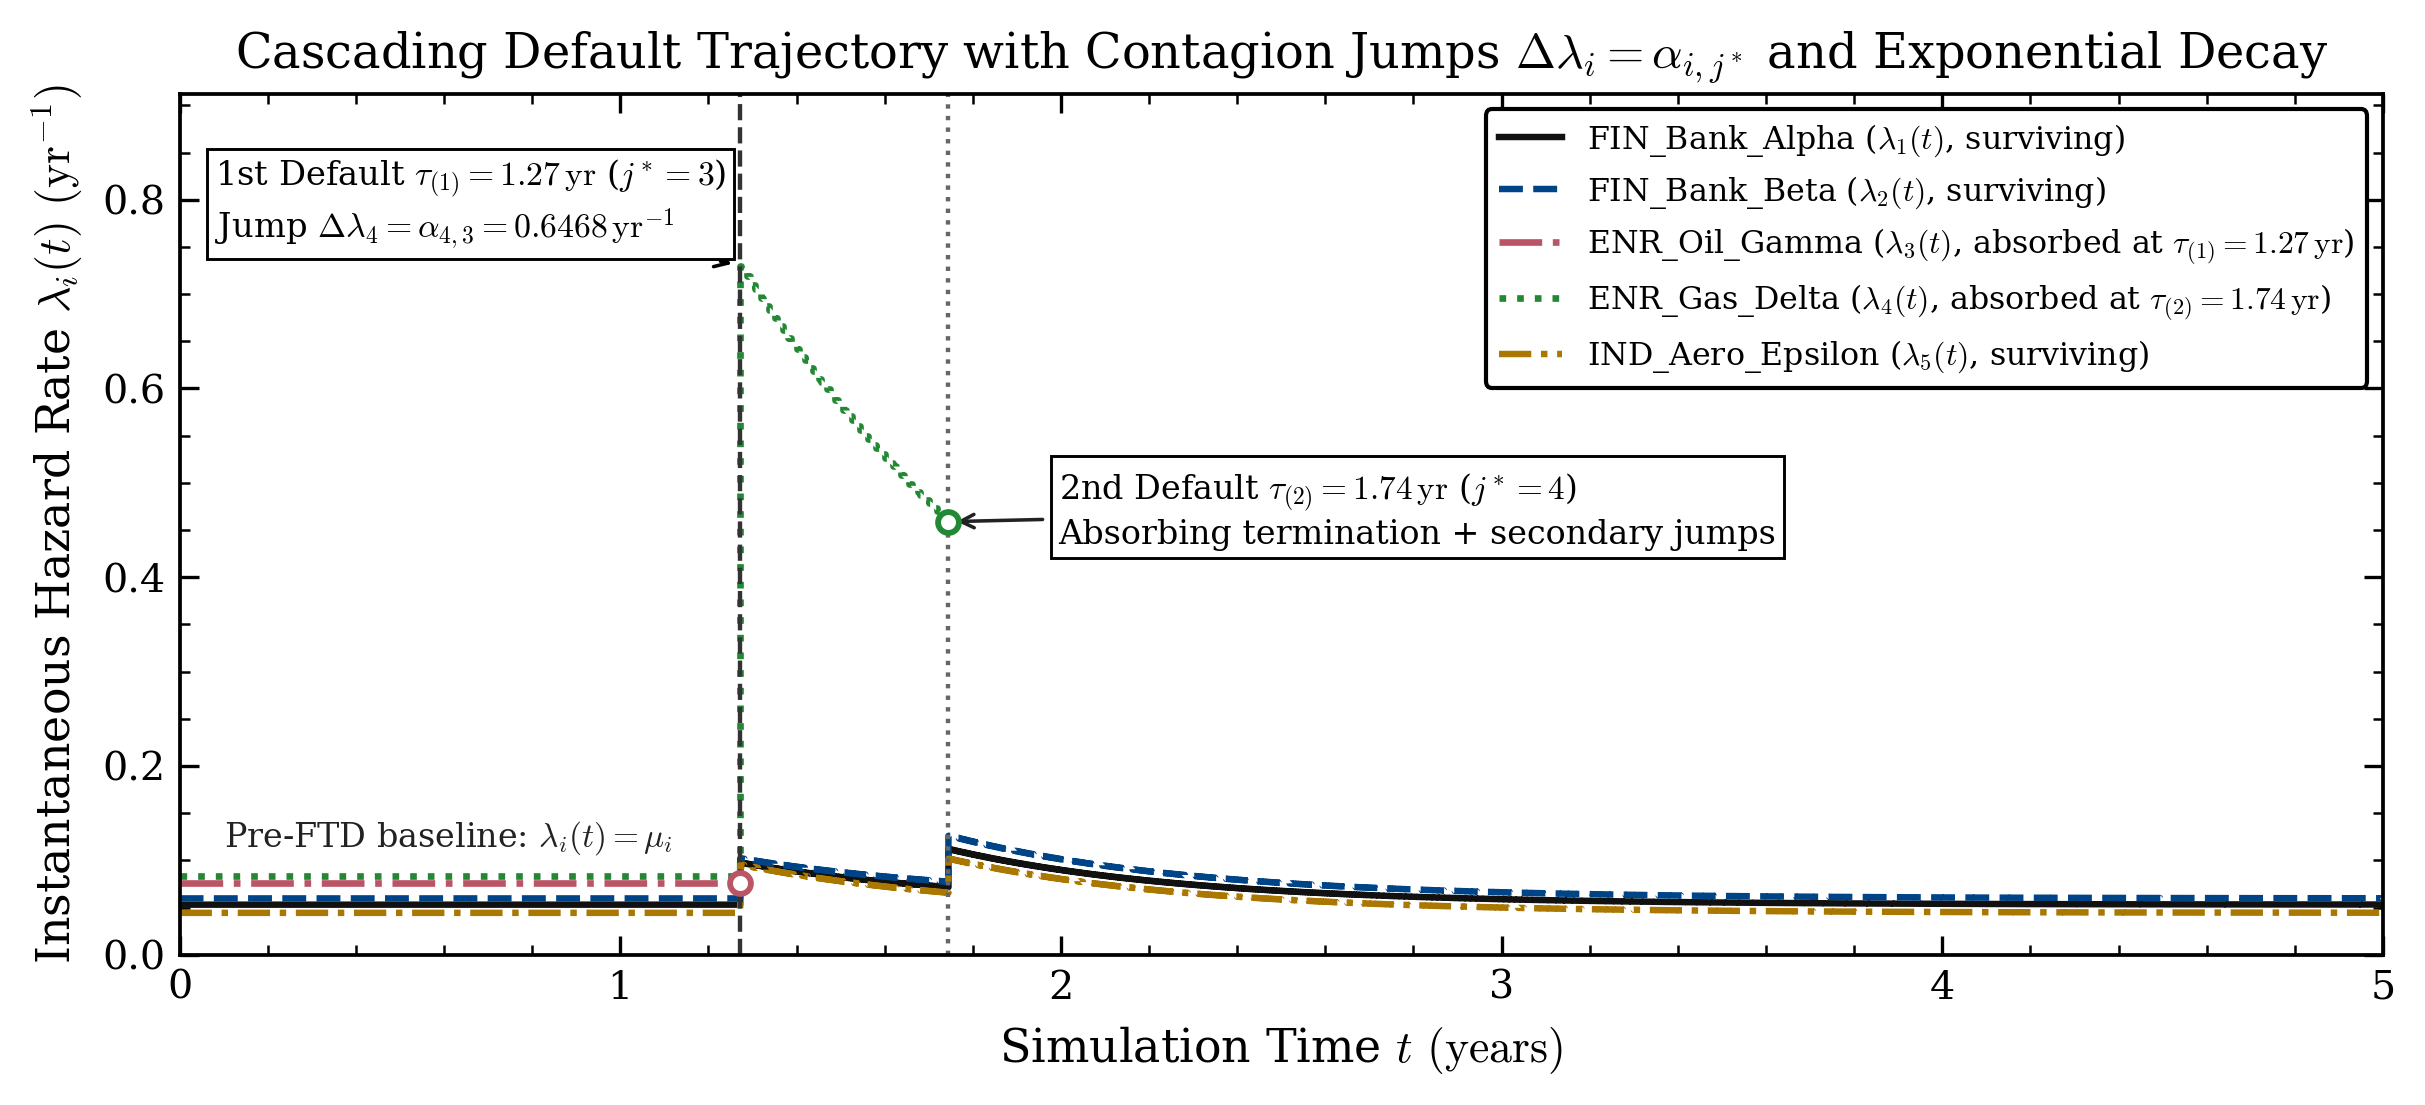
\includegraphics[width=0.98\textwidth]{figures/fig1_cascading_hazard_path.png}
  \caption{A single Monte Carlo trajectory illustrating intra-sector Hawkes contagion. Prior to $\tau_{(1)} = 1.27\text{ yr}$, all five hazard rates sit flat at their baseline values $\lambda_i(t) = \mu_i$. When \texttt{ENR\_Oil\_Gamma} ($j^*=3$) defaults at $\tau_{(1)} = 1.27\text{ yr}$, its own intensity is absorbed while its Energy peer \texttt{ENR\_Gas\_Delta} ($i=4$) experiences an immediate jump $\Delta\lambda_4 = \alpha_{4,3} = 0.6468\text{ yr}^{-1}$, triggering a secondary default at $\tau_{(2)} = 1.74\text{ yr}$.}
  \label{fig:cascading_path}
\end{figure}

\section{Core Modeling Takeaway: Why FTD Swaps Do Not Price Contagion}

Our original project goal was to build a Hawkes Monte Carlo pricer for a \textbf{First-to-Default (FTD)} basket swap ($k=1$) and measure how self-exciting contagion increases the fair FTD spread. When we compared our calibrated Hawkes model ($\alpha_{ij} > 0$) against an independent Poisson baseline ($\alpha_{ij} = 0$), both models produced the exact same fair FTD spread ($1843.11\text{ bps}$).

Inspecting Equation~\eqref{eq:hawkes_intensity} reveals why this is a fundamental mathematical property rather than a bug. An FTD contract terminates at the first default stopping time $\tau_{(1)} = \min_{1 \le i \le N} \tau_i$. For every timestamp $t < \tau_{(1)}$, no default has occurred in the basket, so the counting processes satisfy $N_j(t^-) = 0$ for all $j \in \{1, \dots, N\}$. Consequently, the stochastic contagion integral in Equation~\eqref{eq:hawkes_intensity} vanishes on $[0, \tau_{(1)})$, which reduces each entity's pre-FTD intensity to its constant baseline rate $\lambda_i(t) = \mu_i$ and yields the constant aggregate basket intensity:
\begin{equation}
  \Lambda(t) = \sum_{i=1}^{N} \mu_i \equiv \Lambda_0 \qquad \forall \, t < \tau_{(1)}.
  \label{eq:ftd_invariance}
\end{equation}
Because $\Lambda(t) = \Lambda_0$ is completely independent of $\alpha_{ij}$ and $\beta_{ij}$ prior to $\tau_{(1)}$, the first default time is distributed as $\tau_{(1)} \sim \mathrm{Exponential}\!\left(\sum_{i=1}^N \mu_i\right)$ regardless of how strong post-default contagion is. Furthermore, on the very first step of Ogata's thinning algorithm ($t=0$), the upper bound is $\Lambda^* = \Lambda_0$ and the acceptance probability is $\Lambda(t_{\text{cand}}^-) / \Lambda^* = 1$, so the first exponential draw is always accepted.

\textbf{Takeaway for Credit Structuring}: Self-exciting contagion only activates \emph{at and after} $\tau_{(1)}$. To observe Hawkes excitation repricing basket risk, we must look beyond the $k=1$ equity/FTD tranche to \textbf{$k$-th-to-Default swaps ($k = 2, 3, 4, 5$)}, whose cash flows depend on the conditional waiting times $\tau_{(2)} - \tau_{(1)}, \dots, \tau_{(5)} - \tau_{(4)}$ after the first default shock hits the basket.

\section{Calibration Walkthrough \& Contagion Matrix}

We construct a synthetic 5-name corporate basket distributed across Financials, Energy, plus a single Industrial obligor, evaluated under a constant continuous risk-free rate $r = 4.0\%$ over a $T = 5.0$ year horizon.

\begin{enumerate}
  \item \textbf{Baseline Hazard Rate Bootstrap ($\mu_i$)}: Rather than relying on the rough credit triangle approximation ($\mu_i \approx S_i / \mathrm{LGD}_i$), our routine \texttt{extract\_baseline\_hazard\_rates\_from\_cds} solves the exact quarterly par CDS pricing equation with mid-period accrued premium on default via vectorized fixed-point iteration to $10^{-14}$ tolerance. Repricing the 5-year single-name CDS contracts with the bootstrapped $\mu_i$ recovers the input par spreads to within $10^{-10}\text{ bps}$.
  \item \textbf{Sector Contagion Mapping ($\alpha_{ij}, \beta_{ij}$)}: In \texttt{map\_correlation\_to\_contagion\_matrix}, off-diagonal entries ($i \ne j$) scale pairwise asset correlation $\rho_{ij}^{1.25}$ by source loss severity $\text{LGD}_j / \overline{\text{LGD}}$, weighted by sector co-membership multipliers ($w_{\text{intra}} = 2.40$ for same-sector pairs versus $w_{\text{cross}} = 0.65$ for cross-sector pairs). Intra-sector contagion also decays more slowly ($\beta_{\text{intra}} = 1.15\text{ yr}^{-1}$) than cross-sector spillovers ($\beta_{\text{cross}} = 1.85\text{ yr}^{-1}$). Finally, with $\alpha_{ii} = 0$ fixed on the diagonal, $\boldsymbol{\alpha}$ is scaled so that $\rho(\boldsymbol{\alpha} \oslash \boldsymbol{\beta}) = 0.68$.
\end{enumerate}

\begin{table}[H]
  \centering
  \caption{Synthetic 5-entity credit basket market inputs and bootstrapped baseline hazard rates ($r = 4.0\%$, $T = 5.0\text{ yr}$).}
  \vspace{0.4em}
  \resizebox{\textwidth}{!}{%
  \begin{tabular}{clcccc}
    \toprule
    \textbf{ID} & \textbf{Reference Entity} & \textbf{Sector} & \textbf{5Y CDS Spread (bps)} & \textbf{LGD ($1 - R_i$)} & \textbf{Bootstrapped $\mu_i$ ($\text{yr}^{-1}$)} \\
    \midrule
    $i=1$ & \texttt{FIN\_Bank\_Alpha}   & Financials & $320.0$ & $0.60$ & $0.053067$ \\
    $i=2$ & \texttt{FIN\_Bank\_Beta}    & Financials & $360.0$ & $0.60$ & $0.059701$ \\
    $i=3$ & \texttt{ENR\_Oil\_Gamma}    & Energy     & $420.0$ & $0.55$ & $0.075984$ \\
    $i=4$ & \texttt{ENR\_Gas\_Delta}    & Energy     & $460.0$ & $0.55$ & $0.083220$ \\
    $i=5$ & \texttt{IND\_Aero\_Epsilon} & Industrial & $290.0$ & $0.65$ & $0.044393$ \\
    \midrule
    \multicolumn{3}{l}{\textbf{Pre-FTD Basket Intensity Sum ($\Lambda_0 = \sum_{i=1}^5 \mu_i$)}} & N/A & N/A & $\mathbf{0.316365}$ \\
    \bottomrule
  \end{tabular}%
  }
  \label{tab:calibration}
\end{table}

\begin{figure}[H]
  \centering
  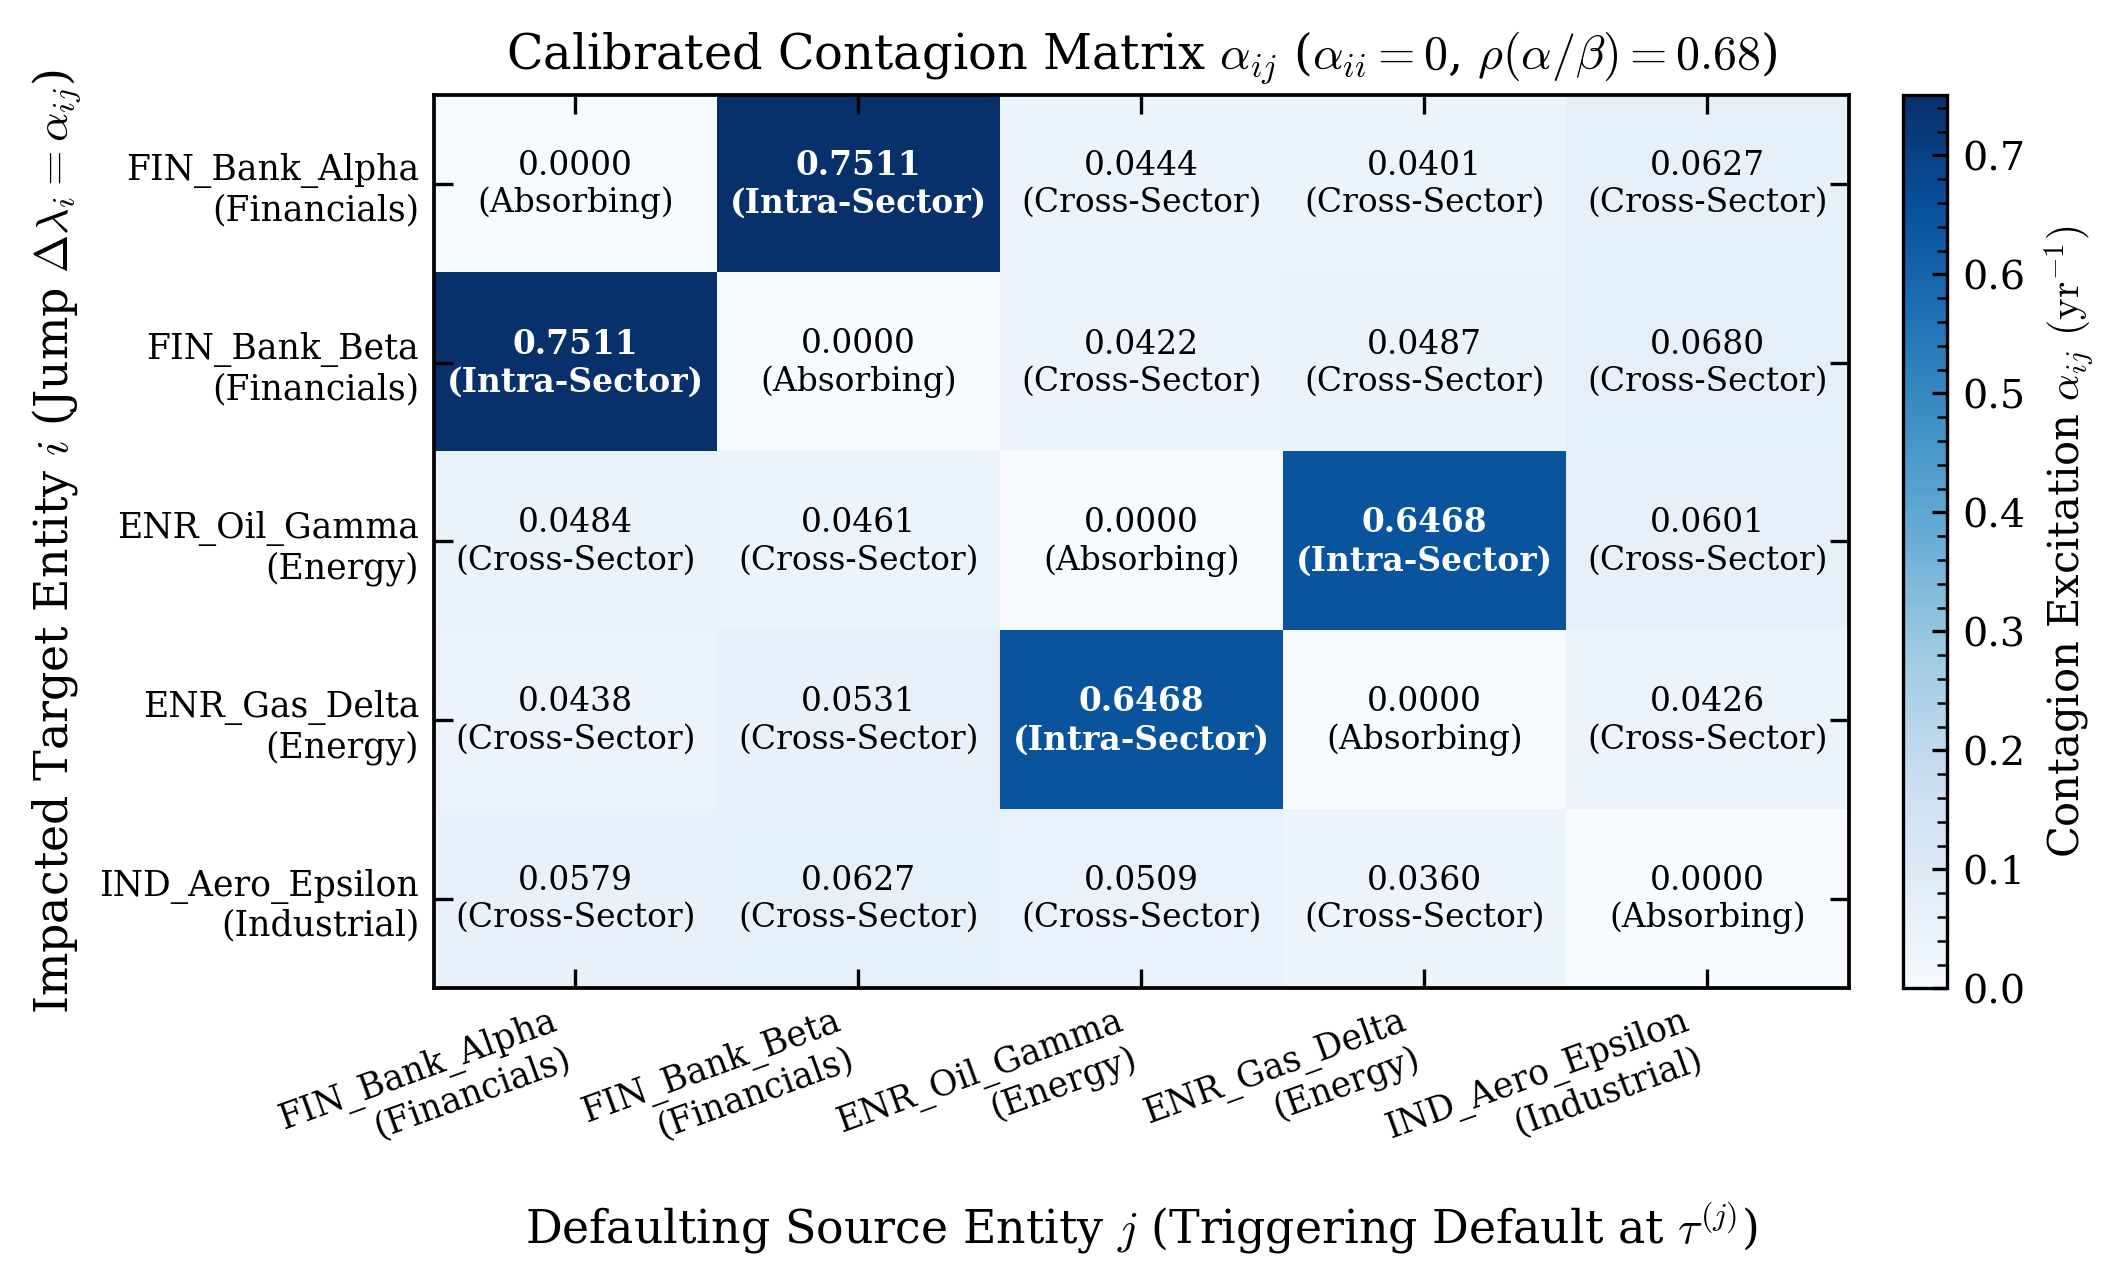
\includegraphics[width=0.86\textwidth]{figures/fig2_contagion_matrix.png}
  \caption{Calibrated Hawkes contagion matrix $\alpha_{ij}$ ($\text{yr}^{-1}$) with absorbing zero diagonal ($\alpha_{ii} = 0$) and spectral radius $\rho(\boldsymbol{\alpha} \oslash \boldsymbol{\beta}) = 0.68$. Intra-sector pairs in Financials ($\alpha_{12}=\alpha_{21}=0.7511$) and Energy ($\alpha_{34}=\alpha_{43}=0.6468$) dominate cross-sector spillovers ($0.0360\text{--}0.0680$).}
  \label{fig:contagion_matrix}
\end{figure}

\section{$k$-th-to-Default Monte Carlo Results \& Implementation Lessons}

For each tranche order $k \in \{1, \dots, 5\}$, the protection buyer pays a continuous spread $S_k$ until $\min(\tau_{(k)}, T)$ in exchange for a payment of $\mathrm{LGD}_{j_{(k)}}$ at $\tau_{(k)}$ if $\tau_{(k)} \le T$. Equating expected discounted leg present values across $M = 10,000$ paths yields the fair spread:
\begin{equation}
  S_k^* = \frac{\mathbb{E}\!\left[\mathbf{1}_{\{\tau_{(k)} \le T\}} \, \mathrm{LGD}_{j_{(k)}} \, e^{-r \tau_{(k)}}\right]}{\mathbb{E}\!\left[\int_0^{\min(\tau_{(k)}, T)} e^{-r t} \, \mathrm{d}t\right]}, \qquad
  \int_0^{\min(\tau_{(k)}, T)} e^{-r t} \, \mathrm{d}t = \frac{1 - e^{-r \min(\tau_{(k)}, T)}}{r}.
\end{equation}

\begin{table}[H]
  \centering
  \caption{$k$-th-to-Default ($k=1,\dots,5$) Monte Carlo pricing comparison across $10,000$ pathwise CRN trajectories (\texttt{seed=42}).}
  \vspace{0.4em}
  \resizebox{\textwidth}{!}{%
  \begin{tabular}{lcccccc}
    \toprule
    \textbf{Tranche} & \textbf{5Y Default Prob.} & \textbf{5Y Default Prob.} & \textbf{Hawkes Spread} & \textbf{Hawkes SE} & \textbf{Indep.\ Spread} & \textbf{Contagion Premium} \\
    \textbf{Order $k$} & \textbf{Hawkes ($\alpha > 0$)} & \textbf{Indep.\ ($\alpha = 0$)} & \textbf{$S_k^*$ (bps)} & \textbf{(bps)} & \textbf{$S_k^{*,0}$ (bps)} & \textbf{$\Delta S_k^*$ (bps)} \\
    \midrule
    $k=1$ (1st TD / FTD) & $79.23\%$ & $79.23\%$ & $1843.11$ & $\pm 20.95$ & $1843.11$ & $\mathbf{0.00}$ \\
    $k=2$ (2nd TD)       & $56.42\%$ & $42.02\%$ & $901.77$  & $\pm 11.37$ & $583.31$  & $\mathbf{+318.47}$ \\
    $k=3$ (3rd TD)       & $28.54\%$ & $12.76\%$ & $368.22$  & $\pm 6.61$  & $149.62$  & $\mathbf{+218.61}$ \\
    $k=4$ (4th TD)       & $11.76\%$ & $1.98\%$  & $137.82$  & $\pm 3.94$  & $22.12$   & $\mathbf{+115.70}$ \\
    $k=5$ (5th TD)       & $2.24\%$  & $0.18\%$  & $25.79$   & $\pm 1.72$  & $2.01$    & $\mathbf{+23.78}$ \\
    \bottomrule
  \end{tabular}%
  }
  \label{tab:kth_results}
\end{table}

\begin{figure}[H]
  \centering
  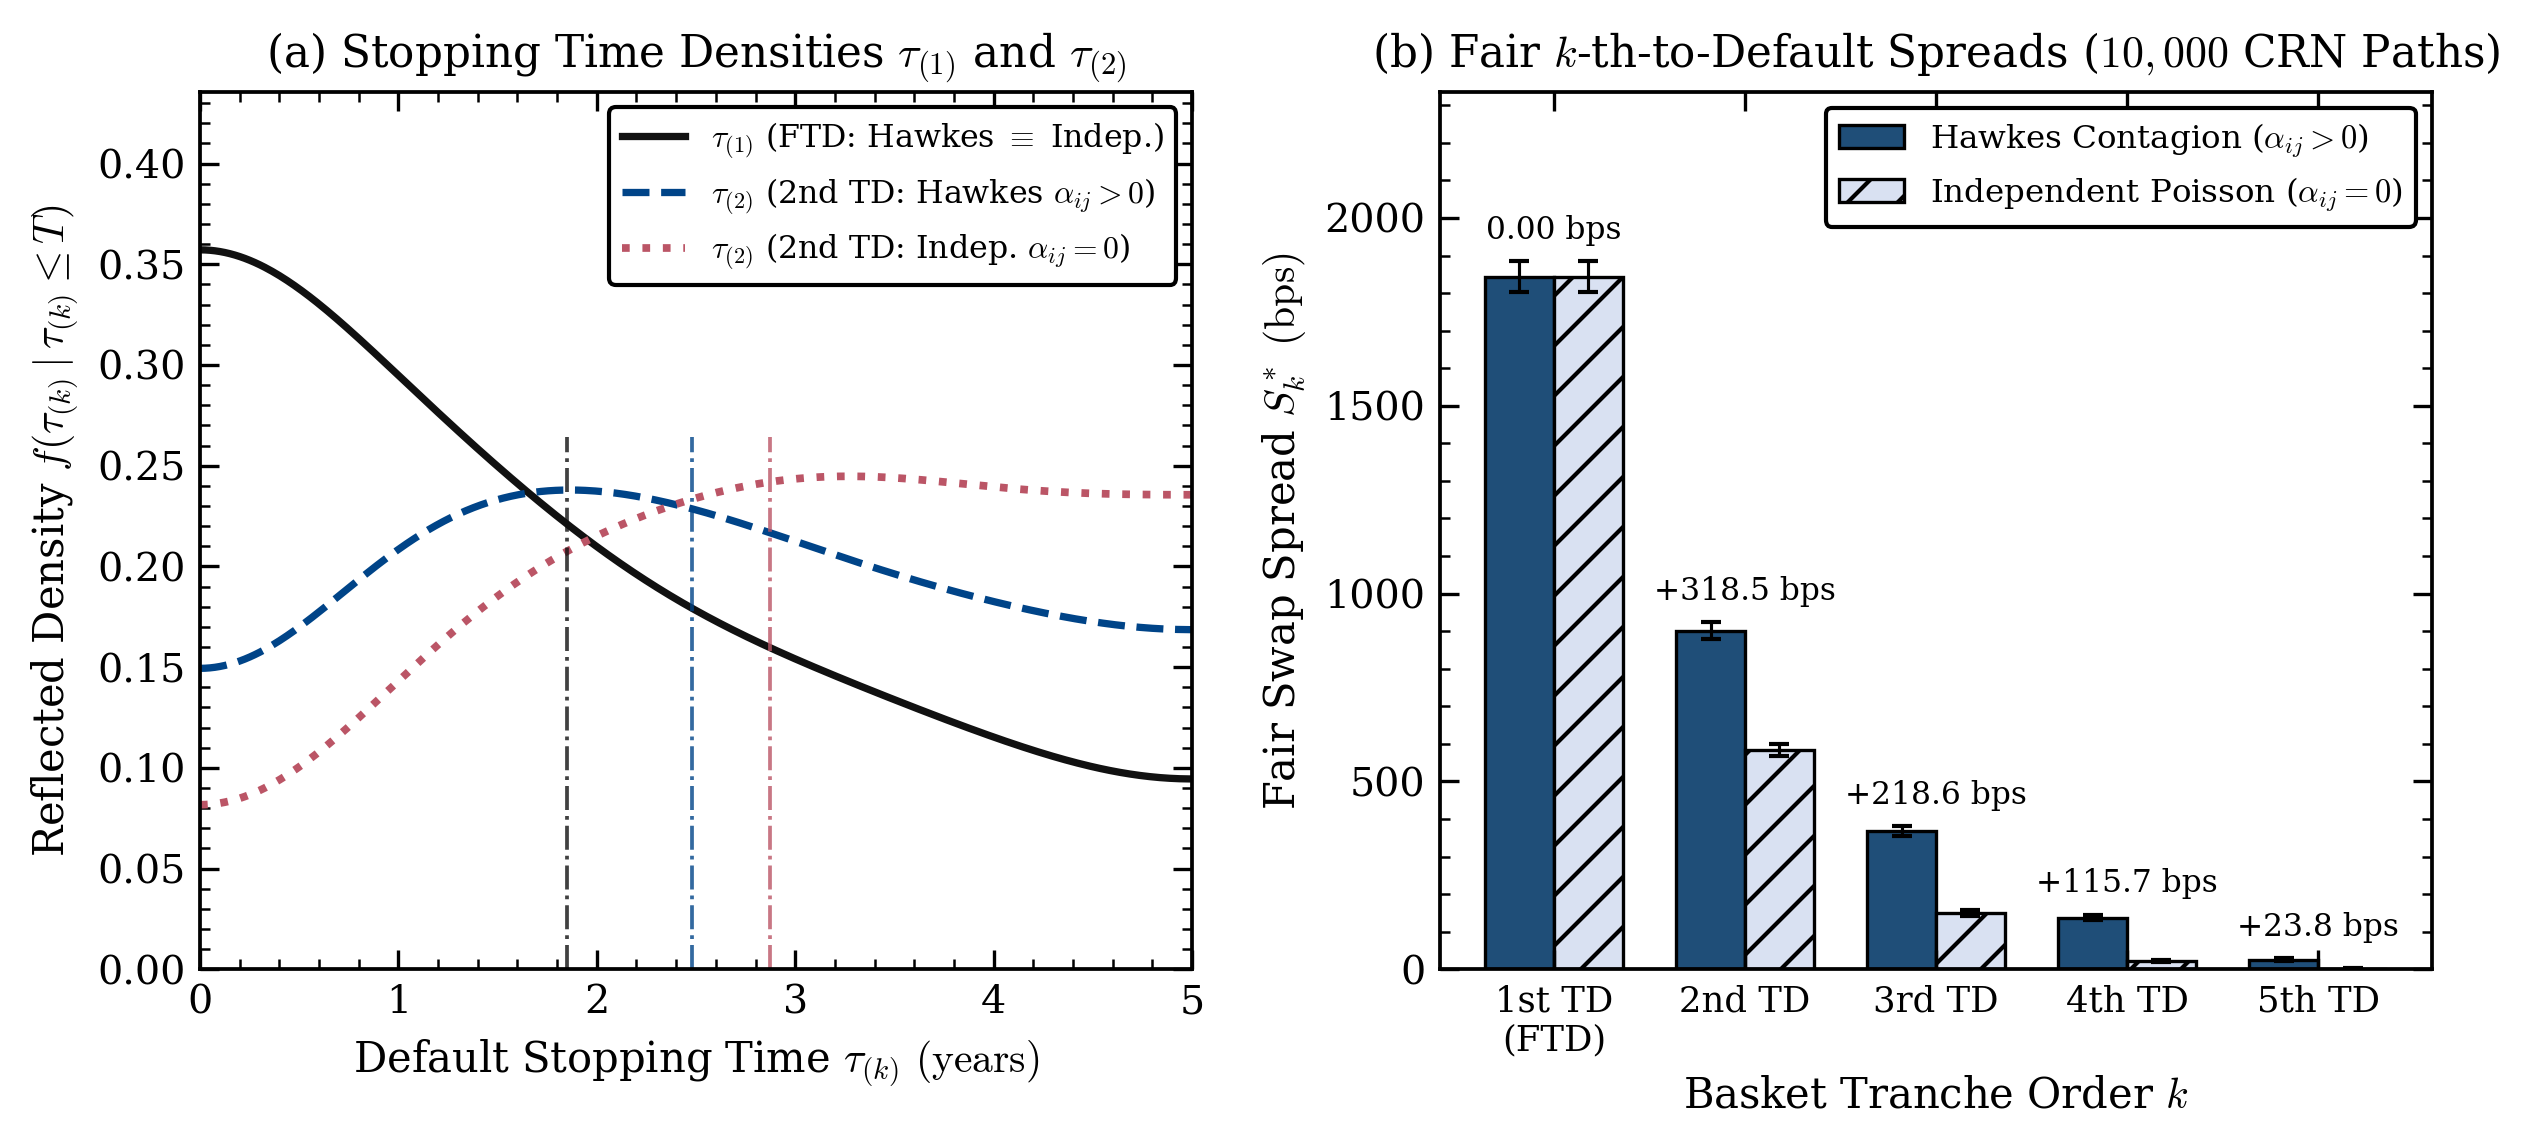
\includegraphics[width=0.99\textwidth]{figures/fig3_kth_default_tranches.png}
  \caption{(a) Boundary-reflected conditional stopping time densities $f(\tau_{(k)} \mid \tau_{(k)} \le T)$ for $\tau_{(1)}$ and $\tau_{(2)}$, with vertical dash-dot lines marking conditional means ($1.85\text{ yr}$ for FTD; $2.48\text{ yr}$ vs.\ $2.88\text{ yr}$ for 2nd TD). (b) Fair $k$-th-to-Default spreads across $k=1,\dots,5$ with $95\%$ confidence intervals and contagion premiums $\Delta S_k^*$.}
  \label{fig:kth_tranches}
\end{figure}

\subsection{Key Implementation Lessons}

\begin{enumerate}
  \item \textbf{Pathwise Common Random Numbers (CRN) via \texttt{SeedSequence.spawn}}: If we simply pass a single global \texttt{np.random.Generator} across all $10,000$ paths, any extra thinning rejection step on path $p$ in the Hawkes model shifts the random number stream for path $p+1$, introducing Monte Carlo noise between the Hawkes and Independent pricers even for $k=1$. Spawning $10,000$ independent child streams via \texttt{SeedSequence(seed).spawn(n\_paths)} isolates each trajectory $p$. Because both models share identical draws up to $\tau_{(1)}$ on every path, CRN locks in $|S_1^{*,\text{Hawkes}} - S_1^{*,\text{Indep}}| < 10^{-12}\text{ bps}$ and sharply reduces the variance of the spread difference $\Delta S_k^*$ for $k \ge 2$.
  \item \textbf{Eliminating KDE Boundary Bias at $t = 0$}: Because $\tau_{(1)} \sim \mathrm{Exponential}(\Lambda_0)$ attains its maximum density at $t = 0$ ($f_{\tau_{(1)}}(0) = \Lambda_0 / (1 - e^{-\Lambda_0 T}) \approx 0.399\text{ yr}^{-1}$), applying a standard Gaussian kernel density estimator directly to positive stopping times $\tau_{(k)} \in [0, T]$ spills half the kernel mass across $t < 0$ and creates an artificial downward hook near $t = 0$. In \texttt{compute\_reflected\_kde}, we reflect the sample across both boundaries (\texttt{np.concatenate([taus, -taus, 2.0 * T - taus])}) and multiply the evaluated density on $[0, T]$ by $3.0$, restoring zero-slope boundary consistency at $t = 0$ and $t = T$.
\end{enumerate}

\end{document}
